\documentclass[10pt,a4paper]{article}
\usepackage{graphicx}
\usepackage{amsmath}
\usepackage{epic}
\usepackage[left=3cm,right=2.5cm,top=2cm,bottom=2cm]{geometry}
\providecommand{\abs}[1]{|#1|}
\title{Pr\'actica Ocho - Elemento finito} 
\author{F\'isica Computacional}
\date{}
%%%%%%%%%%%%%%%%%%%%%%%%%%%%%%%%%%%%%%%%%%%%%%%%%%%%%%%%%%%%%%%%%%%%%%%%%
%%%%%%%%%%%%%%%%%%%%%%%%%%%%%%%%%%%%%%%%%%%%%%%%%%%%%%%%%%%%%%%%%%%%%%%%%
\begin{document}
\thispagestyle{empty}

\vfill
 \begin{center}
    \begin{figure}[h]
    \centering
    \includegraphics[width=12cm]{unsa}\\
    
    \end{figure}
 	 
     \vspace*{1.5cm}
    {\large\bfseries FACULTAD DE PRODUCCIÓN Y SERVICIOS} \\
    {\large\bfseries ESCUELA PROFESIONAL DE CIENCIA DE LA COMPUTACIÓN}  \\    
    \vspace*{1.5cm}
    
 	\rule[0.5ex]{\linewidth}{2pt}\vspace*{-\baselineskip}\vspace*		{3.2pt}
	\rule[0.5ex]{\linewidth}{1pt}\\[\baselineskip]
 	{\huge Física computacional} \\[4mm]
    \rule[0.5ex]{\linewidth}{1pt}\vspace*{-							\baselineskip}\vspace{3.2pt}
	\rule[0.5ex]{\linewidth}{2pt}\\
 	\vspace*{1cm}

    \begin{large} \bfseries
    Práctica 8 - Elemento finito \\
    
    \vspace{5mm}
    Eduardo Antonio Sánchez Hincho \\

    \vspace{5mm}
    Docente:\\
    Edwin Agapito Llamoca Requena
    \end{large}
    \vspace*{0.4in}
    
    \noindent \\
    
    \vfill
    \large\bfseries{ AREQUIPA\\2020}
\end{center}
\newpage


\maketitle

\def\baselinestretch{1.66}
Si queremos aplicar la t\'ecnica del elemento finito debemos de tener un orden muy estricto en el proceso matem\'atico\index{proceso!matem\'atico} y en la secuencia para elaborar el c\'odigo. Para entender bien este m\'etodo le daremos soluci\'on a la ecuaci\'on de Poisson\index{ecuaci\'on!de Poisson} en una dimensi\'on siendo la ecuaci\'on diferencial

\begin{equation}\label{poisson}
  \frac{d^2T}{dx^2}=-f(x)
\end{equation}

\noindent donde $f(x)$ es la funci\'on que define una fuente de calor\index{fuente!de calor} a lo largo de la barra, y los extremos de la barra se mantienen a temperaturas fijas,

$$T(0)=T_1 \hspace*{1.0cm} \mbox { y } \hspace*{1.0cm}  T(L)=T_2$$

Lo que debemos hacer es que la barra la debemos discretizar, es decir dividir en partes iguales y cada parte la llamaremos elemento finito en el que estudiaremos y deduciremos el comportamiento de cada elemento finito. Luego procedemos a ensamblar cada elemento finito para tener toda la barra y por tanto ser\'a la soluci\'on de la ecuaci\'on diferencial\index{ecuaci\'on!diferencial}. En las siguientes secciones veremos la deducci\'on del comportamiento de cada elemento finito.

%%% ----------------------------------------------------------------------
\section{Discretizaci\'on}
Una configuraci\'on simple para modelar la barra calentada es dividir en una serie de elementos de igual longitud. As\'i, el sistema es tratado por ejemplo con diez elementos de igual longitud y once nodos. El efecto de tener una cantidad determinada de elementos y nodos ser\'a relevante para determinar la precisi\'on del m\'etodo. Ahora deduciremos las caracter\'isticas de un elemento finito de cualquier longitud.

%%% ----------------------------------------------------------------------
\section{Funci\'on apropiada para la ecuaci\'on de los elementos}

Primero, debemos elegir una funci\'on apropiada con coeficientes desconocidos, que ser\'a usada para aproximar la soluci\'on. En nuestro caso para una barra calentada unidimensional, la alternativa m\'as simple es un polinomio de primer grado\index{polinomio!de primer grado} de la forma

\begin{equation}\label{Tx}
  P(x) = a_0+a_1x
\end{equation}

Esta funci\'on debe pasar a trav\'es de los valores de $P(x)$ en los puntos extremos del elemento en $x_1$ y $x_2$. Es decir

\begin{equation}\label{Tx1}
  P(x_1) = P_1=a_0+a_1x_1
\end{equation}

\begin{equation}\label{Tx2}
  P(x_2) = P_2=a_0+a_1x_2
\end{equation}

\noindent de aqu\'i determinamos los coeficientes $a_0$ y $a_1$, donde

\begin{equation}\label{a0ya1}
  \displaystyle a_0=\frac{P_1x_2-P_2x_1}{x_2-x_1} \hspace*{0.9cm} \mbox { y } \hspace*{0.6cm} a_1=\frac{P_2-P_1}{x_2-x_1}
\end{equation}

\noindent Estos resultados podemos sustituir en la ecuaci\'on (\ref{Tx}), de manera que

\begin{equation}\label{T}
  P(x) = N_1P_1+N_2P_2
\end{equation}

\noindent donde

\begin{equation}\label{N1yN2}
  \displaystyle N_1(x)=N_1=\frac{x_2-x}{x_2-x_1} \hspace*{0.9cm} \mbox { y } \hspace*{0.6cm} N_2(x)=N_2=\frac{x-x_1}{x_2-x_1}
\end{equation}

La ecuaci\'on (\ref{T}) se conoce como funci\'on de aproximaci\'on\index{funci\'on!aproximaci\'on}, $N_1$ y $N_2$ son funciones de interpolaci\'on de orden uno. La funci\'on de aproximaci\'on (\ref{T}) viene a ser una interpolaci\'on lineal\index{interpolaci\'on lineal} entre las dos temperaturas nodales o extremas del elemento.

%%% ----------------------------------------------------------------------
\section{Funci\'on \'optima\index{funci\'on!\'optima} para la ecuaci\'on de los elementos}

Ahora evaluemos los coeficientes de modo que la funci\'on se aproxime a la soluci\'on de la ecuaci\'on (\ref{poisson}) de manera \'optima. Una vez que eligamos la funci\'on de interpolaci\'on\index{funci\'on!de interpolaci\'on}, debemos desarrollar la ecuaci\'on que determine el comportamiento del elemento. Esta ecuaci\'on representa un ajuste de la funci\'on de la soluci\'on de la ecuaci\'on diferencial (\ref{poisson}). El m\'etodo que vamos a desarrollar para este prop\'osito es el m\'etodo de los residuos ponderados\index{m\'etodo!de los residuos ponderados}. La ecuaci\'on (\ref{poisson}) podemos expresar tambi\'en como 

\begin{equation}\label{qpoisson}
 q=\frac{d^2T}{dx^2}+f(x)
\end{equation}

La soluci\'on aproximada (\ref{T}) podemos sustituir en la ecuaci\'on (\ref{qpoisson}) y no es la soluci\'on exacta porque el lado izquierdo de la ecuaci\'on resultante no ser\'a cero, sino igual a un residuo

\begin{equation}\label{Rpoisson}
 R=\frac{d^2P}{dx^2}+f(x)
\end{equation}
 
El m\'etodo de los residuos ponderados consiste en hallar un m\'inimo para el residuo de acuerdo con la f\'ormula general 

\begin{equation}\label{residuo}
  \displaystyle \int_DRW_idD=0 \hspace*{0.9cm} \mbox { } \hspace*{0.6cm} i=1,2,\dots,n
\end{equation}
 
\noindent donde $D$ es el dominio de la soluci\'on y $W_i$ son las funciones de ponderaci\'on\index{funci\'on!de ponderaci\'on} linealmente independientes. El enfoque m\'as com\'un para el m\'etodo del elemento finito, es emplear las funciones de interpolaci\'on $N_i$ como las funciones de ponderaci\'on. Cuando estas sustituimos en la ecuaci\'on (\ref{residuo}), el resultado es conocido como el m\'etodo de Galerkin\index{m\'etodo!de Galerkin}

\begin{equation}\label{galerkin}
  \displaystyle \int_DRN_idD=0 \hspace*{0.9cm} \mbox { } \hspace*{0.6cm} i=1,2,\dots,n
\end{equation}
 
Si aplicamos en nuestra barra unidimensional, la ecuaci\'on (\ref{Rpoisson}) podemos sustituir en la ecuaci\'on (\ref{galerkin}) para obtener

\begin{equation}\label{i1MRP}
  \displaystyle \int_D\left(\ \frac{d^2P}{dx^2}+f(x) \right)N_idx=0 \hspace*{0.9cm} \mbox { } \hspace*{0.6cm} i=1,2
\end{equation}
 
\noindent donde $N_i$ corresponden a $N_1$ y $N_2$ siendo las funciones de interpolaci\'on de orden uno. Para el dominio tendremos solamente la longitud inicial $x_1$ y final $x_2$ de la barra quedando

\begin{equation}\label{i2MRP}
  \displaystyle \int_{x_1}^{x_2} \frac{d^2P}{dx^2}N_i(x)dx=-\int_{x_1}^{x_2}f(x)N_i(x)dx \hspace*{0.9cm} \mbox { } \hspace*{0.6cm} i=1,2
\end{equation}
 
Simplifiquemos el integrando de lado izquierdo aplicando la integraci\'on por partes al escoger $N_i(x)$  como $u$, y $(d^2P/dx^2)dx$ como $dv$, obtenemos

\begin{equation}\label{i3MRP}
  \displaystyle \int_{x_1}^{x_2} N_i(x)\frac{d^2P}{dx^2}dx=N_i(x) \left . \frac{dP}{dx} \right |_{x_1}^{x_2} -\int_{x_1}^{x_2}\frac{dP}{dx}\frac{dN_i}{dx}dx \hspace*{0.9cm} \mbox { } \hspace*{0.6cm} i=1,2 
\end{equation}

Ahora resolvamos para $i=1$ e $i=2$ la ecuaci\'on (\ref{i3MRP}). Entonces

  \bigskip

{\bf para $i=1$}

  \bigskip

\noindent el primer t\'ermino del lado derecho de la ecuaci\'on (\ref{i3MRP}) escribimos como

\begin{equation}\label{i4MRP}
 N_1(x) \left .\frac{dP}{dx} \right |_{x_1}^{x_2}= N_1(x_2)\left .\frac{dP}{dx}\right |_{x_2}-N_1(x_1)\left .\frac{dP}{dx}\right |_{x_1}
\end{equation}

\noindent de la ecuaci\'on (\ref{N1yN2}) $N_1(x_2)=0$ y $N_1(x_1)=1$, entonces

\begin{equation}\label{i5MRP}
 N_1(x) \left .\frac{dP}{dx} \right |_{x_1}^{x_2}= -\left .\frac{dP}{dx}\right |_{x_1}
\end{equation}

El c\'alculo de la derivada en (\ref{i5MRP}) no se conoce. Reemplazando (\ref{i5MRP}) en (\ref{i3MRP}) y (\ref{i3MRP}) en (\ref{i2MRP}) tenemos

\begin{equation}\label{i6MRP}
 \int_{x_1}^{x_2} \frac{dP}{dx}\frac{dN_1}{dx}dx=-\left .\frac{dP}{dx}\right |_{x_1}+\int_{x_1}^{x_2}f(x)N_1(x)dx 
\end{equation}

Resolvamos ahora la integral de la izquierda de (\ref{i6MRP}). Las derivadas de $P(x)$ y $N_1(x)$ son respectivamente

\begin{equation}\label{dTdx}
  \displaystyle \frac{dP}{dx}=\frac{P_2-P_1}{x_2-x_1} \hspace*{0.9cm} \mbox { y } \hspace*{0.6cm} \frac{dN_1}{dx}=\frac{-1}{x_2-x_1} 
\end{equation}

\noindent luego la primera integral de (\ref{i6MRP}) es

\begin{equation}\label{i7MRP}
 \int_{x_1}^{x_2} \frac{dP}{dx}\frac{dN_1}{dx}dx=\int_{x_1}^{x_2}\frac{P_2-P_1}{x_2-x_1}\frac{-1}{x_2-x_1}dx=\frac{P_1-P_2}{x_2-x_1}
\end{equation}

\noindent entonces

\begin{equation}\label{i1}
 \frac{P_1-P_2}{x_2-x_1}=-\left .\frac{dP}{dx}\right |_{x_1}+\int_{x_1}^{x_2}f(x)N_1(x)dx
\end{equation}

  \bigskip

{\bf para $i=2$}

  \bigskip

\noindent el primer t\'ermino del lado derecho de la ecuaci\'on (\ref{i3MRP}) puede evaluarse como

\begin{equation}\label{i8MRP}
 N_2(x) \left .\frac{dP}{dx} \right |_{x_1}^{x_2}= N_2(x_2)\left .\frac{dP}{dx}\right |_{x_2}-N_2(x_1)\left .\frac{dP}{dx}\right |_{x_2}
\end{equation}

\noindent de la ecuaci\'on (\ref{N1yN2}) $N_2(x_2)=1$ y $N_2(x_1)=0$, entonces

\begin{equation}\label{i9MRP}
 N_2(x) \left .\frac{dP}{dx} \right |_{x_1}^{x_2}= \left .\frac{dP}{dx}\right |_{x_2}
\end{equation}

\noindent reemplazando (\ref{i9MRP}) en (\ref{i3MRP}) y (\ref{i3MRP}) en (\ref{i2MRP}) tenemos

\begin{equation}\label{i10MRP}
 \int_{x_1}^{x_2} \frac{dP}{dx}\frac{dN_2}{dx}dx=\left .\frac{dP}{dx}\right |_{x_2}+\int_{x_1}^{x_2}f(x)N_2(x)dx 
\end{equation}

Resolvamos ahora la integral de la izquierda de (\ref{i10MRP}). Las derivadas de $P(x)$ y $N_2(x)$ son respectivamente

\begin{equation}\label{dTdx_2}
  \displaystyle \frac{dP}{dx}=\frac{P_2-P_1}{x_2-x_1} \hspace*{0.9cm} \mbox { y } \hspace*{0.6cm} \frac{dN_2}{dx}=\frac{1}{x_2-x_1} 
\end{equation}

\noindent luego la primera integral de (\ref{i10MRP}) es

\begin{equation}\label{i11MRP}
 \int_{x_1}^{x_2} \frac{dP}{dx}\frac{dN_2}{dx}dx=\int_{x_1}^{x_2}\frac{P_2-P_1}{x_2-x_1}\frac{1}{x_2-x_1}dx=\frac{P_2-P_1}{x_2-x_1}
\end{equation}

\noindent entonces

\begin{equation}\label{i2}
 \frac{P_2-P_1}{x_2-x_1}=\left .\frac{dP}{dx}\right |_{x_2}+\int_{x_1}^{x_2}f(x)N_2(x)dx
\end{equation}

Los t\'erminos de la izquierda en las ecuaciones (\ref{i1}) y (\ref{i2}) podemos compactar en forma matricial como sigue

\begin{equation*}
 \frac{1}{x_2-x_1}\left[\begin{array}{c}
                              P_1 - P_2 \\
                              P_2 - P_1 
                        \end{array} \right] = \frac{1}{x_2-x_1}\left[\begin{array}{cc}
                                                                            1 & -1 \\
                                                                            -1 & 1 
                                                                     \end{array} \right]
                                                                     \left[\begin{array}{c}
                                                                                 P_1 \\
                                                                                 P_2 
                                                                           \end{array} \right]
\end{equation*}

por tanto, las ecuaciones (\ref{i1}) y (\ref{i2}) escribimos como

\begin{equation}\label{i1i2}
 \frac{1}{x_2-x_1}\left [\begin{array}{cc}
                               1 & -1 \\
                               -1 & 1 
                         \end{array}
                  \right]
                  \left [\begin{array}{c}
                               P_1 \\
                               P_2 
                         \end{array}
                  \right] = \left [\begin{array}{c}
                                        -\left .\frac{dP}{dx}\right |_{x_1} \\
                                                            \\
                                         \left .\frac{dP}{dx}\right |_{x_2}
                                   \end{array}
                            \right] +
                            \left [\begin{array}{c}
                                         \int_{x_1}^{x_2}f(x)N_1(x)dx \\
                                                                      \\
                                         \int_{x_1}^{x_2}f(x)N_2(x)dx
                                   \end{array} \right] 
\end{equation}
La ecuaci\'on (\ref{i1i2}) nos indica que es el comportamiento de cada uno de los elementos de la barra. Adem\'as dichas ecuaciones estan ya minimizadas de acuerdo con (\ref{residuo}), por tanto podemos decir que debe cumplir la ecuaci\'on (\ref{qpoisson}). Finalmente podemos reemplazar $P$ por $T$, siendo
\begin{equation}\label{i1i2final}
 \frac{1}{x_2-x_1}\left [\begin{array}{cc}
                               1 & -1 \\
                               -1 & 1 
                         \end{array}
                  \right]
                  \left [\begin{array}{c}
                               T_1 \\
                               T_2 
                         \end{array}
                  \right] = \left [\begin{array}{c}
                                        -\left .\frac{dT}{dx}\right |_{x_1} \\
                                                            \\
                                         \left .\frac{dT}{dx}\right |_{x_2}
                                   \end{array}
                            \right] +
                            \left [\begin{array}{c}
                                         \int_{x_1}^{x_2}f(x)N_1(x)dx \\
                                                                      \\
                                         \int_{x_1}^{x_2}f(x)N_2(x)dx
                                   \end{array} \right] 
\end{equation}
\noindent que son las ecuaciones de cada uno de los elementos de una barra. Los t\'erminos $T_1$ y $T_2$ es el comportamiento en las fronteras del elemento posicionadas en $x_1$ y $x_2$, respectivamente.

%%% ----------------------------------------------------------------------
\section{Ensamble\index{ensamble}}

La ecuaci\'on del elemento (\ref{i1i2final}) solo esta un funci\'on de los valores en sus fronteras. Es decir, de sus temperaturas y su ubicaci\'on espacial. Lo que se quiere es ensamblar cada de uno de elementos de tal manera que obtengamos toda la barra calentada. Trat\'andose de una barra lineal, el ensamble con cada uno de los elementos es muy simple. El resultado del ensamble se transforma en un conjunto de ecuaciones lineales. Por ejemplo, si la barra se divide en dos elementos iguales, tendr\'iamos 3 ecuaciones lineales cuyas inc\'ognitas son las dos primeras derivadas en la frontera de la barra y la temperatura en el centro de la barra que es el contacto entre el elemento 1 y elemento 2. Las temperaturas encontradas son la soluci\'on de la ecuaci\'on (\ref{poisson}).

Elaboremos un c\'odigo para encontrar la soluci\'on de la ecuaci\'on (\ref{poisson}) mediante elementos finitos. En la figura \ref{gefinito} observamos la alta precisi\'on del m\'etodo de elemento finito comparado con el m\'etodo de Euler con tama\~no de paso $h=0.01$. Para encontrar las temperaturas utilizamos el m\'etodo de Gauss.

\begin{figure}[htb]
  \centering
  \includegraphics[width=130mm,totalheight=90mm]{prg19}
  \caption{Comparaci\'on con diferencias finitas y elementos finitos}
  \label{gefinito}
\end{figure}

  \bigskip

  \hspace*{1cm}{\tt \small{clear, clf, hold on}}

  \hspace*{1cm}{\tt \small{\% resolucion con el metodo de Euler}}

  \hspace*{1cm}{\tt \small{vT = 66; Tp=40; h=0.01;n=0;}}

  \hspace*{1cm}{\tt \small{for x=0:h:10}}

  \hspace*{1.6cm}{\tt \small{n=n+1;}}

  \hspace*{1.6cm}{\tt \small{Tp=Tp+vT*h;}}

  \hspace*{1.6cm}{\tt \small{vT=vT+feval('ddT',x)*h;}}

  \hspace*{1.6cm}{\tt \small{ex(n)=x;}}

  \hspace*{1.6cm}{\tt \small{ey(n)=Tp;}}

  \hspace*{1cm}{\tt \small{end}}

  \hspace*{1cm}{\tt \small{plot (ex,ey,'r');}}

  \hspace*{1cm}{\tt \small{hold on;}}

  \hspace*{1cm}{\tt \small{\% Numero de elementos}}

  \hspace*{1cm}{\tt \small{ne=10;}}

  \hspace*{1cm}{\tt \small{\% Fuente de calor uniforme}}

  \hspace*{1cm}{\tt \small{fu=10;}}

  \hspace*{1cm}{\tt \small{\% Longitud de la barra}}

  \hspace*{1cm}{\tt \small{lb=10;}}

  \hspace*{1cm}{\tt \small{\% Longitud del elemento}}

  \hspace*{1cm}{\tt \small{le=lb/ne;}}

  \hspace*{1cm}{\tt \small{\% Temperatura Inicial}}

  \hspace*{1cm}{\tt \small{Ti=40;}}

  \hspace*{1cm}{\tt \small{\% Temperatura Final}}

  \hspace*{1cm}{\tt \small{Tf=200;}}

  \hspace*{1cm}{\tt \small{\% Numero de nodos}}

  \hspace*{1cm}{\tt \small{\% ------------------------------------------------------------------}}

  \hspace*{1cm}{\tt \small{\% Desarrollar paso a paso y mostrar la matriz mt}}

  \hspace*{1cm}{\tt \small{\% ------------------------------------------------------------------}}

  \hspace*{1cm}{\tt \small{nd=ne+1;}}

  \hspace*{1cm}{\tt \small{mt=0*ones(50,50);}}

  \hspace*{1cm}{\tt \small{bt=0*ones(50);}}

  \hspace*{1cm}{\tt \small{mc(1,1)=+1/le;  mc(1,2)=-1/le;}}

  \hspace*{1cm}{\tt \small{mc(2,1)=-1/le;  mc(2,2)=+1/le;}}

  \hspace*{1cm}{\tt \small{bc(1)=fu*le/2;  bc(2)=fu*le/2;}}

  \hspace*{1cm}{\tt \small{\% ------------------------------------------------------------------}}

  \hspace*{1cm}{\tt \small{\% Mostrar la matriz mc y el vector bc}}

  \hspace*{1cm}{\tt \small{\% ------------------------------------------------------------------}}

  \hspace*{1cm}{\tt \small{for l=0:nd}}

  \hspace*{1.6cm}{\tt \small{for i=1:2}}

  \hspace*{2.2cm}{\tt \small{bt(i+l)=bt(i+l)+bc(i);}}

  \hspace*{2.2cm}{\tt \small{for j=1:2}}

  \hspace*{2.8cm}{\tt \small{mt(i+l,j+l)=mt(i+l,j+l)+mc(i,j);}}

  \hspace*{2.2cm}{\tt \small{end}}

  \hspace*{1.6cm}{\tt \small{end}}

  \hspace*{1cm}{\tt \small{end}}

  \hspace*{1cm}{\tt \small{\% ------------------------------------------------------------------}}

  \hspace*{1cm}{\tt \small{\% Mostrar la matriz mt}}

  \hspace*{1cm}{\tt \small{\% ------------------------------------------------------------------}}

  \hspace*{1cm}{\tt \small{bt(1)=bt(1)-mt(1,1)*Ti;}}

  \hspace*{1cm}{\tt \small{bt(2)=bt(2)-mt(2,1)*Ti;}}

  \hspace*{1cm}{\tt \small{bt(nd)=bt(nd)-mt(nd,nd)*Tf;}}

  \hspace*{1cm}{\tt \small{bt(nd-1)=bt(nd-1)-mt(nd-1,nd)*Tf;}}

  \hspace*{1cm}{\tt \small{mt(1,1)=+1;   mt(2,1)=0;}}

  \hspace*{1cm}{\tt \small{mt(nd,nd)=-1; mt(nd-1,nd)=0;}}

  \hspace*{1cm}{\tt \small{\% ------------------------------------------------------------------}}

  \hspace*{1cm}{\tt \small{\% Mostrar la matriz mt y explique el ensamblaje}}

  \hspace*{1cm}{\tt \small{\% ------------------------------------------------------------------}}

  \hspace*{1cm}{\tt \small{\% fin de desarrollo paso a paso y mostrar la matriz mt}}

  \hspace*{1cm}{\tt \small{\% ------------------------------------------------------------------}}

  \hspace*{1cm}{\tt \small{for k=1:nd-1}}

  \hspace*{1.6cm}{\tt \small{for i=k+1:nd}}

  \hspace*{2.2cm}{\tt \small{factor=mt(i,k)/mt(k,k);}}

  \hspace*{2.2cm}{\tt \small{for j=k+1:nd}}

  \hspace*{2.8cm}{\tt \small{mt(i,j)=mt(i,j)-factor*mt(k,j);}}

  \hspace*{2.2cm}{\tt \small{end}}

  \hspace*{2.2cm}{\tt \small{bt(i)=bt(i)-factor*bt(k);}}

  \hspace*{1.6cm}{\tt \small{end}}

  \hspace*{1cm}{\tt \small{end}}

  \hspace*{1cm}{\tt \small{t(nd)=bt(nd)/mt(nd,nd);}}

  \hspace*{1cm}{\tt \small{for i=nd-1:-1:1}}

  \hspace*{1.6cm}{\tt \small{sum=0;}}

  \hspace*{1.6cm}{\tt \small{for j=i+1:nd}}

  \hspace*{2.2cm}{\tt \small{sum=sum+mt(i,j)*t(j);}}

  \hspace*{1.6cm}{\tt \small{end}}

  \hspace*{1.6cm}{\tt \small{t(i)=(bt(i)-sum)/mt(i,i);}}

  \hspace*{1cm}{\tt \small{end}}

  \hspace*{1cm}{\tt \small{t(1)=Ti;  t(nd)=Tf;}}

  \hspace*{1cm}{\tt \small{lf=0; k=1;}}

  \hspace*{1cm}{\tt \small{for i=1:ne}}

  \hspace*{1.6cm}{\tt \small{cx(i) = lf;}}

  \hspace*{1.6cm}{\tt \small{cy(i) = t(i);}}

  \hspace*{1.6cm}{\tt \small{lf=lf+le;}}

  \hspace*{1cm}{\tt \small{end}}

  \hspace*{1cm}{\tt \small{cx(ne+1)=lf;}}

  \hspace*{1cm}{\tt \small{cy(ne+1)=t(nd);}}

  \hspace*{1cm}{\tt \small{grid on;}}

  \hspace*{1cm}{\tt \small{plot (cx,cy);}}

  \hspace*{2cm}{\tt \small{xlabel('Distancia de la barra');}}

  \hspace*{2cm}{\tt \small{ylabel('Temperatura';}}
  
\section{Desarrollo a mano\index{desarrolloAMano}}
\begin{figure}[H]
    \centering
    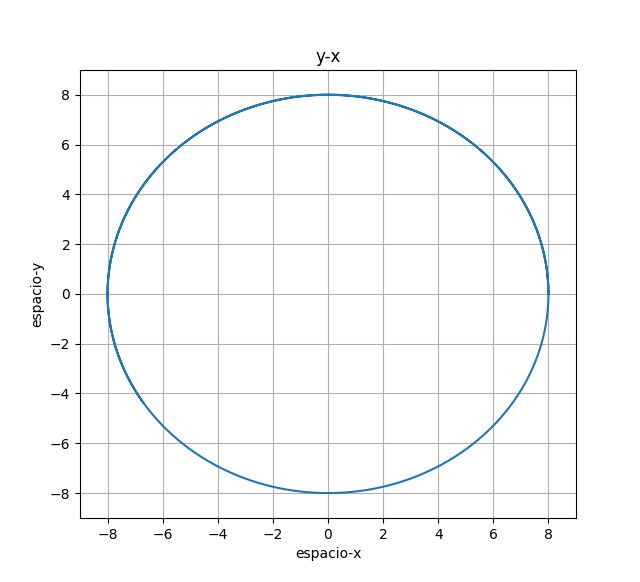
\includegraphics[width=1\textwidth]{1.jpg}
    \caption{Resultado}
\end{figure}
\begin{figure}[H]
    \centering
    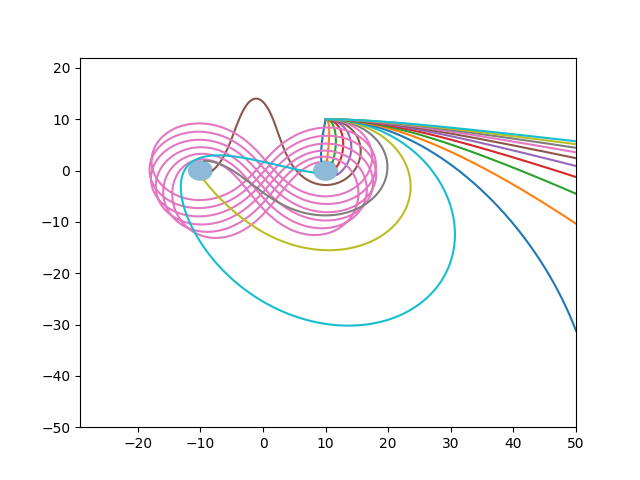
\includegraphics[width=1\textwidth]{2.jpg}
    \caption{Resultado}
\end{figure}
\begin{figure}[H]
    \centering
    \includegraphics[width=1\textwidth]{3.jpg}
    \caption{Resultado}
\end{figure}
\begin{figure}[H]
    \centering
    \includegraphics[width=1\textwidth]{4.jpg}
    \caption{Resultado}
\end{figure}


 
 \end{document}
